\documentclass[10pt]{article}
\pdfoutput=1
%\usepackage{NotesTeX,lipsum}
\usepackage{NotesTeX,lipsum}
%\usepackage{showframe}

\title{\begin{center}{\Huge \textit{Notes}}\\{{\itshape Something}}\end{center}}
\author{Yi Huang}


\affiliation{
University of Minnesota
}

\emailAdd{yihphysics@gmail.com}

\begin{document}
	\maketitle
	\flushbottom
	\newpage
	\pagestyle{fancynotes}
	\part{Caprice}
	\section{Fall 2018}\label{sec:fall2018}
	\begin{margintable}\vspace{.8in}\footnotesize
		\begin{tabularx}{\marginparwidth}{|X}
		Section~\ref{sec:fall2018}. Fall 2018\\
		\end{tabularx}
	\end{margintable}

	This is my note for some non-trivial but not systematic problems which involves some interesting physics or maths.

	\subsection{Walkway equilibrium}

	Suppose the mass of the objects attached to each end of the rope are $m_1$ and $m_2$, The angles between each segment of the rope, bended by the central object which has mass $M$, with the horizontal plane are $\theta$ and $\phi$. The distance between two pulleys is $L$, and what we want to know is the vertical displacement $d$ of the central object. Thus we can obtaind the equations for $d$ when the system is at equilibrium.
	\begin{gather}
		L = d (\cot \theta + \cot \phi), \label{eq: total L}\\
		m_1 g \cos \theta = m_2 \cos \phi, \label{eq: Tx}\\
		m_1 g \sin \theta + m_2 g \sin \phi = Mg, \label{eq: Ty}
	\end{gather}
	From \eqref{eq: Tx}, we have $\cos \phi = \tfrac{m_1}{m_2} \cos \theta$, thus \eqref{eq: Ty} can be written as
	\begin{equation}
		m_1 \sin \theta + m_2 \sqrt{1 - \tfrac{m_1^2}{m_2^2}(1- \sin^2 \theta)} = M,
	\end{equation}
	such that we can solve for $\sin \theta$ and $\cos \theta$
	\begin{gather}
		\sin \theta = \frac{M^2 + m_1^2 - m_2^2}{2 M m_1}, \\
		\cos \theta = \sqrt{1 - \sin^2 \theta} = \frac{1}{2 M m_1} \sqrt{[(m_1 + m_2)^2 - M^2][M^2 - (m_1 - m_2)^2]}, \\
		\cot \theta = \frac{\sqrt{[(m_1 + m_2)^2 - M^2][M^2 - (m_1 - m_2)^2]}}{M^2 + m_1^2 - m_2^2},
	\end{gather}
	together with $\sin \phi$ and $\cos \phi$
	\begin{gather}
		\cos \phi = \frac{m_1}{m_2} \cos \theta = \frac{1}{2 M m_2} \sqrt{[(m_1 + m_2)^2 - M^2][M^2 - (m_1 - m_2)^2]}, \\
		\sin \phi = \sqrt{1 - \cos^2 \phi} = \frac{M^2 - m_1^2 + m_2^2}{2M m_2}, \\
		\cot \phi = \frac{\sqrt{[(m_1 + m_2)^2 - M^2][M^2 - (m_1 - m_2)^2]}}{M^2 - m_1^2 + m_2^2}.
	\end{gather}
	Therefore we can plug into \eqref{eq: total L} and obtain the expression of $d$ as follows
	\begin{equation}
		d = \frac{L[M^4 - (m_1^2 - m_2^2)^2]}{2M^2 \sqrt{[(m_1 + m_2)^2 - M^2][M^2 - (m_1 - m_2)^2]}}.
	\end{equation}
	The equilibrium condition in this case is
	\begin{equation}
		\abs{m_1 - m_2} < M < (m_1 + m_2).
	\end{equation}
	such that the argument under the square root is positive. Also we can easily check that if $m_1 = m_2 = m$ then this result reduces to our former result
	\begin{equation}
		d = \frac{L M}{2\sqrt{4m^2 - M^2}}.
	\end{equation}

	\subsection{A derivation of Gamma function from Fourier transfrom}

	It is well-known that $\Gamma(n+1) = n!$ for any natural number $n \in \mathbb{N}$. It is natural to ask what is $\Gamma(x)$ for any real number $x \ge 1$. Our purpose is to show that Gamma function can be express as an integral
	\begin{equation}
		\Gamma(x) = \int_0^{\infty} \dd{x} t^{x-1} \e^t, \label{eq: gamma integral}
	\end{equation}
	given that
	\begin{equation}
		\Gamma(x+1) = x \Gamma(x), \label{eq: gamma recursion}
	\end{equation}
	which is the most essential property and motivation to define the Gamma function.

	Using Talor expansion we can easily show that
	\begin{equation}
		f(x + \Delta x) = \sum_{n=0}^{\infty} \frac{f^{(n)}(x)}{n!} (\Delta x)^n = \exp(\Delta x \dv{x}) f(x)
	\end{equation}
	where $\Delta x$ is a constant of translation. Therefore $\Gamma(x + 1) = \e^{\dv{x}} \Gamma(x)$, and we can rewrite \eqref{eq: real gamma recursion} as
	\begin{equation}
		\e^{\dv{x}} \Gamma(x) = x \Gamma(x). \label{eq: real gamma recursion}
	\end{equation}
	Consider doing Fourier transform of \eqref{eq: real gamma recursion}, such that $\dv{x} \to i \omega$, $x \to i \dv{\omega}$, $\Gamma(x) \to \tilde{\Gamma}(\omega)$, and
	\begin{gather}
		\tilde{\Gamma}(\omega) = \mathcal{F}[\Gamma(x)] = \int_{-\infty}^{\infty} \dd{x} \Gamma(x) \e^{-i \omega x}, \\
		\Gamma(x) = \mathcal{F}^{-1}[\tilde{\Gamma}(\omega)] = \int_{-\infty}^{\infty} \frac{\dd{\omega}}{2 \pi} \tilde{\Gamma}(\omega) \e^{i \omega x}, \\
		\e^{i \omega} \tilde{\Gamma}(\omega) = i \dv{\omega} \tilde{\Gamma}(\omega).
	\end{gather}
	Solve the above differential equation of $\tilde{\Gamma}(\omega)$ we find
	\begin{gather}
		\tilde{\Gamma}(\omega) = C \exp(- \e^{i \omega}), \label{eq: real gamma} \\
		\Gamma(x) = \int_{-\infty}^{\infty}  \frac{\dd{\omega}}{2 \pi} C \exp(- \e^{i \omega}) \e^{i \omega x}. \label{eq: inverse fourier gamma in real}
	\end{gather}
	However, \eqref{eq: inverse fourier gamma in real} does not converge, since \eqref{eq: real gamma} is a nonzero periodic function.

	To resolve this difficulty of convergence, we expand the domain of Gamma function to the complex plane, such that $\Gamma(z + 1) = z \Gamma(z)$, where $z \in \mathbb{C}$. Consider a pure imaginary number $z = i x$, where $x \in \mathbb{R}$, we can rewrite the recursion relation \eqref{eq: gamma recursion} as
	\begin{equation}
		\e^{-i \dv{x}} \Gamma(ix) = ix \Gamma(ix)
	\end{equation}
	Again using Fourier transform we have
	\begin{equation}
		\e^{\omega} \mathcal{F}[\Gamma(ix)] = - \dv{\omega} \mathcal{F}[\Gamma(ix)], \label{eq: pure imaginary gamma}
	\end{equation}
	where $\mathcal{F}[\Gamma(ix)]$ is the Fourier transform of $\Gamma(ix)$
	\begin{equation}
		\mathcal{F}[\Gamma(ix)] = \int_{-\infty}^{\infty} \dd{x} \Gamma(ix) \e^{- i \omega x}.
	\end{equation}
	Solve \eqref{eq: pure imaginary gamma} we have
	\begin{gather}
		\mathcal{F}[\Gamma(ix)] = C \exp(- \e^{\omega}), \\
		\Gamma(ix) = \frac{C}{2\pi} \int_{-\infty}^{\infty} \dd{\omega} \exp(- \e^{\omega}) \e^{i \omega x}.
	\end{gather}
	Thus
	\begin{align*}
		\Gamma(z) &= \frac{C}{2\pi} \int_{-\infty}^{\infty} \dd{\omega} \exp(- \e^{\omega}) \e^{\omega z} \\
		&= \frac{C}{2\pi} \int_{-\infty}^{\infty} \dd{\e^{\omega}} \exp(- \e^{\omega}) \e^{\omega (z-1)} \\
		&= \frac{C}{2\pi} \int_{-\infty}^{\infty} \dd{t} t^{z-1} \e^{-t}.
	\end{align*}
	To determine the constant $C$ we use the fact that $\Gamma(1) = 0! = 1$, thus $C/2\pi = 1$, and we obtain the final integral expression of Gamma function
	\begin{equation}
		\Gamma(z) = \int_{-\infty}^{\infty} \dd{t} t^{z-1} \e^{-t}
	\end{equation}
	where $z \in \mathbb{C}$.

	\subsection{Euler's reflection formula}

	In mathematics, a reflection formula or reflection relation for a function f is a relationship between $f(a-x)$ and $f(x)$. A famous relationship is Euler's reflection formula
	\begin{proposition}\label{prop: Euler's reflection formula}
		\begin{equation}
			\Gamma(z)\Gamma(1-z) = \frac{\pi}{\sin{\pi z}}\qc z \not \in \mathbb{Z}.
		\end{equation}
	\end{proposition}
	\begin{proof}
		To prove this reflection formula, we first notice a relationship between Gamma function and Beta function
		\begin{equation}
			B(q, p) = \frac{\Gamma(q) \Gamma(p)}{\Gamma(q + p)},
		\end{equation}
		where
		\begin{equation}
			B(q, p) = \int_0^1 \dd{t} t^{q-1} (1-t)^{p-1} \qc q,p \neq 0, -1, -2, \dots
		\end{equation}
		This can be shown by performing a variable transformation of $\Gamma(q) \Gamma(p)$
		\begin{align*}
			\Gamma(q) \Gamma(p) &= \int_0^{\infty} \dd{u} \e^{-u} u^{q-1} \int_0^{\infty} \dd{v} \e^{-v} v^{p-1} \\
			u = zt, v = z(1-t)\qc &= \int \dd{z} \dd{t} \abs{\pdv{(u,v)}{(z,t)}} \e^{-z} (zt)^{q-1} [z(1-t)]^{p-1} \\
			&= \int_0^{\infty} \dd{z} z^{q+p-1} \e^{-z} \int_0^1 \dd{t} t^{q-1} (1-t)^{p-1} \\
			&= \Gamma(q+p) B(q, p).
		\end{align*}
		Therefore
		\begin{equation}
			\Gamma(z)\Gamma(1-z) = B(z, 1-z) = \int_0^1 \dd{t} t^{z-1} (1-t)^{-z}.
		\end{equation}
		In order to prove Proposition \ref{prop: Euler's reflection formula}, we only need to prove
		\begin{equation}
			\int_0^1 \dd{t} t^{z-1} (1-t)^{-z} = \frac{\pi}{\sin{\pi z}}.
		\end{equation}
		Perform a variable substitution $t \to \frac{x}{1+x}$, such that $\dd{t} = \dd{x}/(1+x)^2$ and
		\begin{equation}
			\int_0^1 \dd{t} t^{z-1} (1-t)^{-z} = \int_0^{\infty} \dd{x} \frac{x^{z-1}}{1+x}
		\end{equation}
		Consider the following integral
		\begin{equation}
			\int_0^{\infty} \dd{x} \frac{x^{\alpha-1}}{x+\e^{i \phi}}\qc 0<\alpha<1\qc -\pi<\phi<\pi.
		\end{equation}
	\end{proof}

	\subsection{$\chi^2$ distribution with $(n-1)$ degrees of freedom}

	Let $Y_1, Y_2, \dots, Y_n$ be independent random variables with $\E(Y_i) = \mu$ and $V(Y_i) = \sigma^2$ for $i = 1,2,\dots,n$. Let
	\begin{equation}
		U_1 = \sum_{i = 1}^n a_i Y_i \qand U_2 = \sum_{i=1}^n b_i Y_i,
	\end{equation}
	where $a_1, a_2, \dots, a_n$, and $b_1, b_2, \dots, b_n$ are constants. $U_1$ and $U_2$ are said to be orthogonal if $\Cov(U_1, U_2) = 0$.

	\begin{enumerate}
		\item Show that $U_1$ and $U_2$ are orthogonal if and only if $\sum_{i=1}^n a_i b_i = 0$.
		\begin{proof}
			Sufficiency: If $\sum_{i=1}^n a_i b_i = 0$, then
			\begin{align*}
				\Cov(U_1, U_2) &= \E\bqty{\qty(\sum_{i = 1}^n a_i Y_i)\qty(\sum_{j=1}^n b_j Y_j)} - \E\qty(\sum_{i = 1}^n a_i Y_i) \E\qty(\sum_{j=1}^n b_j Y_j) \\
				&= \sum_{i=1}^n a_i b_i [\E(Y_i^2) - \E(Y_i)^2] + \sum_{i \neq j} a_i b_j [\E(Y_i Y_j) - \E(Y_i) \E(Y_j)] \\
				&= \sigma^2 \sum_{i=1}^n a_i b_i = 0.
			\end{align*}
			Thus $U_1$ and $U_2$ are orthogonal.
			Necessity: If $U_1$ and $U_2$ are orthogonal, $\Cov(U_1, U_2) = \sigma^2 \sum_{i=1}^n a_i b_i = 0$, then we must have $\sum_{i=1}^n a_i b_i = 0$ if $\sigma \neq 0$.
		\end{proof}
		\item Show that if each component of independent random variables $Y_1, Y_2, \dots, Y_n$ is normally distributed, then any linear combination $U = a_1 Y_1 + a_2 Y_2 + \dots + a_n Y_n$ is normally distributed.
		\begin{proof}
			Proof by induction. We begin with two independent random variables $X_1 = a_1 Y_1 \sim N(\mu_1, \sigma_1^2)$, $X_2 = a_2 Y_2 \sim N(\mu_2, \sigma_2^2)$, with $\mu_i = a_i \mu$ and $\sigma_i^2 = a_i^2 \sigma^2$. Their sum $Z = a_1 Y_1 + a_2 Y_2$, which is a linear combination of $Y_1$ and $Y_2$.
			The characteristic function
			\begin{equation}
				\varphi_Z(t) = \varphi_{X_1 + X_2}(t) = \E(\e^{i t (X_1 + X_2)})
			\end{equation}
			of the sum of two independent random variables is just the product of the characteristic functions of each random variable
			\begin{equation}
				\varphi_{X_1 + X_2}(t) = \varphi_{X_1}(t) \varphi_{X_2}(t) = \E(\e^{i t X_1}) \E(\e^{i t X_2}).
			\end{equation}
			The characteristic function of the normal distribution with expected value $\mu$ and variance $\sigma^2$ is
			\begin{equation}
				\varphi(t) = \exp[it\mu - \tfrac{1}{2} \sigma^2 t^2].
			\end{equation}
			Thus
			\begin{align*}
				\varphi_{X_1 + X_2}(t) &= \exp[it\mu_1 - \tfrac{1}{2} \sigma_1^2 t^2] \exp[it\mu_2 - \tfrac{1}{2} \sigma_2^2 t^2] \\
				&= \exp[it(\mu_1 + \mu_2) - \tfrac{1}{2} (\sigma_1^2 + \sigma_2^2) t^2].
			\end{align*}
			This is the characteristic function of the normal distribution with expected value $(\mu_1 + \mu_2)$ and variance $(\sigma_1^2 + \sigma_2^2)$. Finally, recall that no two distinct distributions can both have the same characteristic function, so the distribution of $Z$ must be just this normal distribution.

			Similarly we can prove that $W = Z + X_3$, which is a linear combination of $Y_1, Y_2$ and $Y_3$, is also normally distributed. By induction, we prove that every linear combination of $Y_1, Y_2, \dots, Y_n$ is normally distributed.
		\end{proof}
		\item Suppose, in addition, that $Y_1, Y_2, \dots, Y_n$ have a multivariate normal distribution. Then $U_1$ and $U_2$ have a bivariate normal distribution. Show that $U_1$ and $U_2$ are independent if they are orthogonal.
		\begin{proof}
			If the random vector $\vb{Y} = (Y_1, Y_2, \dots, Y_n)^\top$ have the multivariate normal distribution, then every linear combination of its components $U = a_1 Y_1 + a_2 Y_2 + \dots + a_n Y_n$ is normally distributed. By definition, since the linear combination of $U_1$ and $U_2$ is still a linear combination of $\vb{Y}$, thus $c_1 U_1 + c_2 U_2$ is normally distributed, and we say $U_1$ and $U_2$ have a bivariate normal distribution.

			In general the bivariate density function of two random variables $Y_1$ and $Y_2$ has the following form
			\begin{equation}
				f(y_1, y_2) = \frac{\e^{-Q/2}}{2\pi \sigma_1 \sigma_2 \sqrt{1-\rho^2}} \qc -\infty < y_1, y_2 < \infty,
			\end{equation}
			where
			\begin{equation}
				Q = \frac{1}{1-\rho^2} \bqty{\frac{(y_1 - \mu_1)^2}{\sigma_1^2} - 2\rho \frac{(y_1 - \mu_1)(y_2 - \mu_2)}{\sigma_1 \sigma_2} + \frac{(y_2 - \mu_2)^2}{\sigma_2^2}}.
			\end{equation}
			By doing a tedious integral exercise, we find $\Cov(Y_1, Y_2) = \rho \sigma_1 \sigma_2$. If $\Cov(Y_1, Y_2) = 0$, i.e. if $\rho = 0$, then
			\begin{equation}
				f(y_1, y_2) = g(y_1) h(y_2),
			\end{equation}
			where $g(y_1)$ is a nonnegative function of $y_1$ alone and $h(y_2)$ is a nonnegative function of $y_2$ alone. Therefore, if $U_1$ and $U_2$ are orthogonal, i.e. $\Cov(U_1, U_2) = 0$, then $U_1$ and $U_2$ are independent. Notice that in general $\Cov(U_1, U_2) = 0$ doesn't imply $U_1$ and $U_2$ are independent. It is only in the context of bivariate normal distribution that we have this conclusion.
		\end{proof}
	\end{enumerate}

	Suppose that $Y_1, Y_2, \dots, Y_n$ is a random sample from a normal distribution with mean $\mu$ and variance $\sigma^2$. The independence of $\sum_{i=1}^n (Y_i - \overline{Y})^2$ and $\overline{Y}$ can be shown as follows. Define an $n \times n$ matrix $A$ by
	\begin{equation}
		A =
		\begin{bmatrix}
			\frac{1}{\sqrt{n}} & \frac{1}{\sqrt{n}} & \frac{1}{\sqrt{n}} & \frac{1}{\sqrt{n}} & \cdots & \frac{1}{\sqrt{n}} & \frac{1}{\sqrt{n}} \\
			\frac{1}{\sqrt{2}} & \frac{-1}{\sqrt{2}} & 0 & 0 & \cdots & 0 & 0 \\
			\frac{1}{\sqrt{2 \cdot 3}} & \frac{1}{\sqrt{2 \cdot 3}} & \frac{-2}{\sqrt{2 \cdot 3}} & 0 & \cdots & 0 &0 \\
			\vdots & \vdots & \vdots & \vdots & \vdots & \vdots & \vdots \\
			\frac{1}{\sqrt{(n-1)n}} & \frac{1}{\sqrt{(n-1)n}} && \cdots && \frac{1}{\sqrt{(n-1)n}} & \frac{-(n-1)}{\sqrt{(n-1)n}}
		\end{bmatrix}
	\end{equation}
	and notice that $A^\top A = I$, the identity matrix. Then,
	\begin{equation}
		\sum_{i = 1}^n Y_i^2 = \vb{Y}^{\top} \vb{Y} = \vb{Y}^{\top} A^{\top} A \vb{Y},
	\end{equation}
	where $\vb{Y}$ is the vector of $Y_i$ values.
	\begin{enumerate}
		\item Show that
		\begin{equation}
			A \vb{Y} =
			\begin{bmatrix}
				\overline{Y} \sqrt{n} \\
				U_1 \\
				U_2 \\
				\vdots \\
				U_{n-1}
			\end{bmatrix}.
		\end{equation}
		where $U_1, U_2, \dots, U_{n-1}$ are linear funcitions of $Y_1, Y_2, \dots, Y_n$. Thus,
		\begin{equation}
			\sum_{i=1}^n Y_i^2 = n \overline{Y}^2 + \sum_{i=1}^{n-1} U_i^2.
		\end{equation}
		\item Show that the linear functions $\overline{Y} \sqrt{n}, U_1, U_2, \dots, U_{n-1}$ are pairwise orhogonal and hence independent under the normality assumption.
		\begin{proof}
			Notice that the coefficients of $\overline{Y}$ and $U_i$ are the elements of each row of matrix $A$, such that
			\begin{gather}
				A = \bmqty{\vb{a}_0^{\top} \\ \vb{a}_1^{\top} \\ \vb{a}_2^{\top} \\ \vdots \\ \vb{a}_{n-1}^{\top}}\qc
				\overline{Y} = \vb{a}_0^{\top} \vb{Y}\qc
				U_i = \vb{a}_i^{\top} \vb{Y}.
			\end{gather}
			Since $\vb{a}_i^{\top} \vb{a}_j = \delta_{ij}$, $\overline{Y} \sqrt{n}, U_1, U_2, \dots, U_{n-1}$ are pairwise orthogonal. In addition, $\vb{Y}$ has a multivariate normal distribution, because every linear combination of its components is normally distributed. Recall the previous exercise, if the multivariate normal distribution $\overline{Y} \sqrt{n}, U_1, U_2, \dots, U_{n-1}$ are pairwise orthogonal, then they are independent random variables.
		\end{proof}
		\item Show that
		\begin{equation}
			\sum_{i=1}^n (Y_i - \overline{Y})^2 = \sum_{i=1}^{n-1} U_i^2
		\end{equation}
		and conclude that this quantity is independent of $\overline{Y}$.
		\begin{proof}
			\begin{align*}
				\sum_{i=1}^n (Y_i - \overline{Y})^2 &= \sum_{i=1}^n (Y_i^2 - 2Y_i\overline{Y} + \overline{Y}^2) \\
				&= \sum_{i=1}^n Y_i^2 - n \overline{Y}^2 \\
				&= \vb{Y}^{\top} A^{\top} A \vb{Y} - n \overline{Y}^2 \\
				&=
				\begin{bmatrix}
					\overline{Y} \sqrt{n}, &
					U_1, &
					U_2, &
					\cdots, &
					U_{n-1}
				\end{bmatrix}
				\begin{bmatrix}
					\overline{Y} \sqrt{n} \\
					U_1 \\
					U_2 \\
					\vdots \\
					U_{n-1}
				\end{bmatrix} - n \overline{Y}^2 \\
				&= \sum_{i=1}^{n-1} U_i^2
			\end{align*}
			Since $U_i$ is independent of $\overline{Y}$, $\sum_{i=1}^{n-1} U_i^2$ is also independet of $\overline{Y}$.
		\end{proof}
		\item Using the results of part (3), show that
		\begin{equation}
			\frac{\sum_{i=1}^n (Y_i - \overline{Y})^2}{\sigma^2} = \frac{(n-1)S^2}{\sigma^2} \label{eq: chi squared n-1 df}
		\end{equation}
		has a $\chi^2$ distribution with $(n-1)$ df.
		\begin{proof}
			First we show that $U_i \sim N(0, \sigma^2)$, and thus $Z_i = U_i/\sigma \sim N(0, 1)$, a standard normal distribution.

			We have seen from the previous exercise that any linear combination of independent random variables with normal distribution is also normally distributed, so $U_i$ has normal distribution, with expected value
			\begin{equation}
				\E(U_i) = \mu \norm{\vb{a}_i}_1 = 0,
			\end{equation}
			and variance
			\begin{equation}
				\Var(U_i) = \sigma^2 \norm{\vb{a}_i}_2^2 = \sigma^2.
			\end{equation}

			Next we prove that if each $Z_i$ is independent with standard normal distribution, then $\sum_{i = 1}^n Z_i^2$ has a $\chi^2$ distribution with $n$ df.

			The characteristic function of $Z_i^2$ is
			\begin{align*}
				\varphi_{Z_i^2}(t) &= \E\qty(\e^{it Z_i^2}) \\
				&= \int_{-\infty}^{\infty} \dd{z} \frac{1}{\sqrt{2\pi}} \e^{it z^2} \e^{-z^2/2} \\
				&= (1 - 2it)^{-1/2},
			\end{align*}
			and from the fact that $Z_i$ is independent with each other, the characteristic function of $V = \sum_{i = 1}^n Z_i^2$ is the product of $n$ characteristic functions of $Z_i^2$
			\begin{equation}
				\varphi_{V}(t) = \prod_{i=1}^n \varphi_{Z_i^2}(t) = (1 - 2it)^{-n/2}
			\end{equation}
			Because characteristic functions are unique, $V$ has a $\chi^2$ distribution with $n$ degrees of freedom.

			Finally we prove that $\sum_{i=1}^n (Y_i - \overline{Y})^2/\sigma^2$ has a $\chi^2$ distribution with $n$ df. We rewrite the \eqref{eq: chi squared n-1 df} as follows
			\begin{equation}
				\frac{\sum_{i=1}^n (Y_i - \overline{Y})^2}{\sigma^2} = \frac{\sum_{i=1}^{n-1} U_i^2}{\sigma^2} = \sum_{i=1}^{n-1} Z_i^2.
			\end{equation}
			Thus it has a $\chi^2$ distribution with $(n-1)$ degrees of freedom.
		\end{proof}
	\end{enumerate}

	\subsection{Exam 08}

	\begin{exercise}
		Suppose that $X_1, X_2, \dots, X_n, X_{n+1}, \dots, X_{n+m}$ is a random sample from a normal distribution $N(0, \sigma^2)$.
		\begin{enumerate}
			\item Find $a$ and $b$ such that
			\begin{equation}
				V = a\qty(\sum_{i=1}^n X_i)^2 + b\qty(\sum_{i=n+1}^{n+m} X_i)^2
			\end{equation}
			has a $\chi^2$ distribution.
			\begin{solution}
				Any linear combination of independent normally distributed random variables is also a random variable with normal distribution. Therefore
				\begin{equation}
					Z_1 = \frac{\sum_{i=1}^n X_i}{\sigma \sqrt{n}} \qc Z_2 = \frac{\sum_{i=n+1}^{n+m} X_i}{\sigma \sqrt{m}}.
				\end{equation}
				Both $Z_1$ and $Z_2$ have standard normal distributions $N(0,1)$. Thus
				\begin{equation}
					a\qty(\sum_{i=1}^n X_i)^2 + b\qty(\sum_{i=n+1}^{n+m} X_i)^2 = a n \sigma^2 Z_1^2 + b m \sigma^2 Z_2^2.
				\end{equation}
				If $a = 1/n\sigma^2$ and $b = 1/m\sigma^2$, then $V = Z_1^2 + Z_2^2$ has a $\chi^2$ distribution with 2 df.
			\end{solution}

			\item Find $c$ such that
			\begin{equation}
				U = \frac{c \sum_{i=1}^n X_i}{\sqrt{\sum_{i=n+1}^{n+m} X_i^2}}
			\end{equation}
			has a $t$ distribution.

			\begin{solution}
				Recall the definition of $t$ distribution
				\begin{definition}
					Let $Z$ be a standard normal random variable and let $W$ be a $\chi^2$-distributed variable with $\nu$ df. Then, if $Z$ and $W$ are independent,
					\begin{equation*}
						T = \frac{Z}{\sqrt{W/\nu}}
					\end{equation*}
					is said to have a $t$ distribution with $\nu$ df.
				\end{definition}
				From part (1) we know that
				\begin{equation}
					Z_1 = \frac{\sum_{i=1}^n X_i}{\sigma \sqrt{n}}
				\end{equation}
				has a standard normal distribution. In additon
				\begin{equation}
					W = \sum_{i=n+1}^{n+m} (\frac{X_i}{\sigma})^2
				\end{equation}
				is a $\chi^2$-distributed variable with $m$ df. Thus
				\begin{align*}
					U &= \frac{c \sum_{i=1}^n X_i}{\sqrt{\sum_{i=n+1}^{n+m} X_i^2}} \\
					&= c \sqrt{\frac{n}{m}} \frac{Z_1}{\sqrt{W/m}}.
				\end{align*}
				If $c = \sqrt{m/n}$, then $U$ is a $t$-distributed variable with $m$ df.
			\end{solution}
		\end{enumerate}
	\end{exercise}

	\subsection{Shape of water in a rotating bucket}

	This is a static equilibrium problem in a rotating frame. Suppose the rotating bucket with radius $R$ has an constant angular velocity $\omega$. When the system arrives equilibrium, the differential volume element of the water will have the same angular velocity $\omega$. We can write down its action in cylindrical coordinates
	\begin{align*}
		S &= \int_{t_0}^{t_1} \dd{t} \int_{V} \dd{r}^3 \mathscr{L}(t, r, z) \\
		&= \const \int_M \dd{m} (\frac{1}{2} v^2 - g z) \\
		&\propto \int_{0}^{R} \dd{r} 2 \pi r z(r) \qty[\frac{1}{2} \omega^2 r^2 - \frac{1}{2} g z(r)] \\
		&\propto \int_{0}^{R} \dd{r} \qty(\omega^2 r^3 z - g r z^2),
	\end{align*}
	where $z(r)$ is the shape of the water, $\mathscr{L}$ is the Lagrangian density. There is an additional constraint of $z(r)$ for the conservation of volume
	\begin{equation}
		\int_0^R \dd{r} 2 \pi r z(r) = V = \const
	\end{equation}
	So we have variation problem with additional condition. It is easy to solve using Lagrange multipliers' method. Necessary condition for $S$ to have extrema is existing a multiplier $\lambda$ such that
	\begin{gather}
		F = \omega^2 r^3 z - g r z^2 + \lambda r z, \\
		\dv{r} \pdv{F}{\pdv{z}{r}} - \pdv{F}{z} = 0.
	\end{gather}
	Since $F$ does not depend on $\pdv{z}{r}$ explicitly, we obtain
	\begin{equation}
		\omega^2 r^3 - 2 g r z + \lambda r = 0,
	\end{equation}
	or equivalently
	\begin{equation}
		z = \frac{\omega^2 r^2}{2g} + \lambda,
	\end{equation}
	where $\lambda$ is determined by
	\begin{gather*}
		\int_0^R \dd{r} 2 \pi r z(r) = \frac{\pi \omega^2 R^4}{4g} + \lambda \pi R^2 = V, \\
		\lambda = \frac{V}{\pi R^2} - \frac{\omega^2 R^2}{4 g}.
	\end{gather*}

\subsection{Derivative of inverse function}

Suppose we are given a function $f$ with its invers $f^{-1}$. Using a little geometry, we can compute the derivative $\dv*{f^{-1}(x)}{x}$ in terms of $f$. See Fig(\ref{fig: 1}).

\begin{figure}[H]
	\centering
	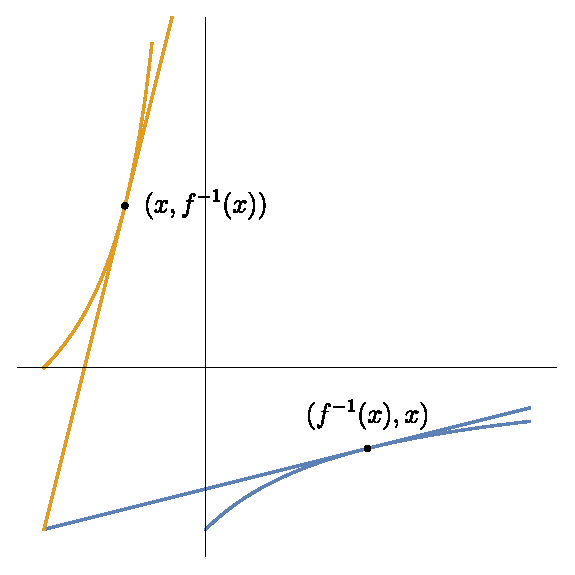
\includegraphics[height = 7cm]{./graphs/inverse_function.eps}
	\caption{A schematic picture for function$f$ and its inverse $f^{-1}$. The slopes at points $(f^{-1}(x),x)$ and $(x,f^{-1}(x))$ are reciprocal to each other.}
	\label{fig: 1}
\end{figure}

Hence we have
\begin{equation}
	\dv{f^{-1}(x)}{x} = 1\Big{/}\eval{\dv{f(x')}{x'}}_{x' = f^{-1}(x)}.
\end{equation}

\begin{example}
	\begin{align*}
		\dv{x} \arcsin{x} &= 1\Big{/}\eval{\dv{x'} \sin{x'}}_{x' = \arcsin{x}} \\
		&= \frac{1}{\eval{\cos{x'}}_{x' = \arcsin{x}}} \\
		&= \frac{1}{\eval{\sqrt{1-\sin^2{x'}}}_{x' = \arcsin{x}}} \\
		&= \frac{1}{\sqrt{1-x^2}}.
	\end{align*}
\end{example}

\subsection{s-wave scattering and zero energy bound states}
We look at a rectangular potential which is attractive
\begin{equation}
	V(r) =
	\begin{cases}
			-V_0,& r<r_0 \\
			0,& r>r_0
	\end{cases}.
\end{equation}
where $V_0 >0$. For low energy, we focus on s-wave scattering. Inside the potential the wave function $u(r) = r A_0(r) \to 0$, as $r\to 0$, because $A_0(r)$ must be finite at $r = 0$. Hence
\begin{equation}
	u(r) = A \sin(k'r),
\end{equation}
where $k' = \sqrt{2m(E+V_0)/\hbar^2}$ is the wave number inside the potential. Outside the potential we have a phase shift $\delta_0$, so we have
\begin{equation}
	u(r) = B \sin(kr + \delta_0),
\end{equation}
where $k = \sqrt{2mE/\hbar^2}$ is the wave number outside the potential. Next we match the boundary conditions
\begin{align*}
	A \sin(k'r_0) &= B \sin(kr_0 + \delta_0), \\
	A k' \cos(k' r_0) &= B k \cos(kr_0 + \delta_0).
\end{align*}
Devide the two equations above we have
\begin{equation}
	\tan(kr_0 + \delta_0) = \frac{k}{k'} \tan{k' r_0},
\end{equation}
or
\begin{equation}
	\delta_0 = -kr_0 + \tan^{-1}\qty(\frac{k}{k'}\tan(k'r_0)).
\end{equation}

\end{document}
